%!TEX root = ../thesis.tex
%*******************************************************************************
%*********************************** First Chapter *****************************
%*******************************************************************************

\chapter{Getting started}  %Title of the First Chapter

\ifpdf
    \graphicspath{{Chapter1/Figs/Raster/}{Chapter1/Figs/PDF/}{Chapter1/Figs/}}
\else
    \graphicspath{{Chapter1/Figs/Vector/}{Chapter1/Figs/}}
\fi


%********************************** %First Section  **************************************
\section{Introduction} 
On the 30th of August 1958, famous statistician Ronald A. Fisher wrote a letter to the journal \textit{Naure} critiquing the evidence linking smoking to lung cancer. The reasons he cited for his suspicions reflect a wider challenge in biomedical research. In his letter, RA Fisher mentioned that causality is difficult to establish from observational data that show increased rates of lung cancer among smokers. Since then, a huge body of literature established the causal link between smoking and lung cancer (reviewed in \cite{Malone2012-na}), but the problems of causal inference in biology and public health remain alive \cite{Glass2013-up}. Reproducible associations between observed exposures and outcomes have often not withstood more robust experimental designs such as randomised controlled trials. This is often attributed to several limitations of observational data, including confounding, reverse causation, and measurement errors. Confounding manifests as an observed association between an exposure and an outcome that results from a confounding factor that is associated with both. Reverse causation happens when the direction of effect is not clear between an exposure and an outcome.\\

Over the last 15 years, genome-wide association studies have provided thousands of associations between genetic variants and outcomes of interest. A significant difference between GWAS and epidemiological studies is that variants do not suffer from the same problems of observational data. Genetic variants are rarely confounded by social, behavioural or environmental factors. Moreover, genetic variants are determined at conception and do not therefore suffer from reverse causation in the same way that observed exposures do \cite{Smith2007-py}. GWASes have typically used a case-control study design to uncover genetic variants associated with different traits and diseases. As the sample sizes of these studies increased, it became apparent that a large number of genetic loci underpin most complex traits and diseases. These findings naturally posed several questions: which effector genes are targeted by these risk-modulating genetic variants? Which biological pathways do they implicate? What can these findings tell us about disease pathogenesis? These questions are not unique to genetics research. They are important from biological, clinical and drug development perspectives. However, genetics offers a unique angle to answer these questions by minimising the risk of associations driven by confounding and reverse causality, something that is difficult to guard against when researchers make conclusions about disease biology in \textit{in vivo} and \textit{in vitro} studies. 

\subsection{Two major gaps in the post-GWAS area}
Trait and disease GWASes are often cited as an example of successful population-scale genetics endeavors. The majority of GWASes recruited tens of thousands of disease cases and controls to identify genetic variants that are enriched in disease cases compared to healthy controls. These efforts have revealed that disease-associated genetic variants are significantly enriched in non-coding sequences such as enhancers, open chromatin regions, and chromatin markers \cite{Ahonen2009-eo,Degner2012-dq,Trynka2013-qs}. 

The difficulty of interpreting GWAS results heralded several important "post-GWAS" approaches to understand the effects of genetic variation. The overall theme of these approaches is to bridge the wide gap between genetic variation and the end phenotypes under investigation. At the molecular end of this gap is understanding the molecular effects of disease-associated variants. At the phenotype end is to understand how genetic variation predisposes to various disease subphenotypes. In this context, the aim of this thesis it improve our understanding of the effects of genetic variation at these two levels. At the molecular level, a better understanding should improve our ability to understand the biological pathways affected by disease-associated genetic variation, and how these effects manifest in different contexts. At the disease subphenotype level, a better understanding of the genetic determinants of disease subphenotypes will help us explain the heterogeneity of disease manifestations in complex diseases. 

% make better use of both the powerful GWAS study design and the advances in high-throughput molecular assay techniques developed over the last decade. 
% Despite the success of GWASes in identifying disease-associated loci, there are two main gaps in genetics research in what can be called the "post-GWAS era". The success of GWASes is often 


\subsection{Why splicing?}
The majority of disease-associated variants are located in the non-coding genome \cite{Hindorff2009-te}. This has made the interpretation of their downstream functional effects difficult. To help bridging this gap, population-level molecular studies that map genetic variation to variation in molecular traits has been set up (molecular quantitative trait loci or mQTLs). mQTLs reveal how genetic variation regulates different molecular traits, and in doing so can help us link genetically regulated molecular variation to disease risk. 

In eukaryotic cells, biological functions are exerted as a complex coordinated program where cells produce effector molecules to exert various functions. These functions aim to sustain cell growth, enable cells to perform their functions or respond to external environmental cues. This process encompasses a wide range of molecular steps that start by gene expression and end with translation to effector proteins and different post-translation modifications. The range of genetically regulated molecular traits is therefore wide and includes chromatin accessibility, methylation, gene expression, post-transcriptional modifications, protein levels and post-trasnlational protein modifications. Several studies have investigated the genetic determinants of methylation QTLs \cite{Oliva2023-nt,Hannon2016-mt,Morrow2018-fv,Taylor2019-tm,Huan2019-ke,Andrews2017-os}, chromatin accessibility QTLs \cite{Alasoo2018-pv,Currin2021-kp}, expression QTLs \cite{The_GTEx_Consortium2020-gg,Vosa2021-pb,Kerimov2021-gh}, splicing QTLs \cite{The_GTEx_Consortium2020-gg,Qi2022-iz}, and protein QTLs \cite{Yao2018-oy,Sun2018-uy} in a wide range of cell types and tissues. Although DNA provides a fixed blueprint for cellular function, different molecular aspects of cellular functions are highly dependent on the environmental context of each cell. Moreover, the genetic regulation of molecular traits has also been shown to vary between tissues, cell types and even environmental contexts \cite{Zhernakova2017-uo,Mu2021-ar}. Profiling mQTLs in relevant contexts has also been shown to improve the ability to explain the functional effects of disease-associated variants \cite{Ongen2017-cd}.\\

Despite the large number of mQTLs, expression QTLs remain the most comprehensively characterised type of mQTLs. The rapid development of RNA-seq methods, both at the experimental and analytical levels, have accelerated the identification of eQTLs in large numbers of tissues and cell types. eQTLs have been succesfully used to identify effector genes for several complex diseases. For example, using pancreatic islet QTLs Viñuela et al. robustly linked 22 Type 2 diabetes loci to effector genes \cite{Vinuela2020-ce}. Although eQTLs have been extensively catalogued in many cell types and tissues, almost 50\% of GWAS loci are still unexplained by eQTLs \cite{Mountjoy2021-fc}. This gap is at least partly attributed to the lack of diversity of of other types of mQTLs. Relative to eQTLs, fewer studies have comprehensively catalogued the several post-transcriptional steps that follow gene expression.\\

Alternative splicing (AS) is a widespread co-transcriptional modification, whereby intronic sequences are removed from transcribed mRNA and exonic sequences form mature mRNA transcripts. Since its discovery in the 1970s, our appreciation of the role of AS in eukaryotic gene expression has increased. Due to their limited scope, earlier transcriptomic profiling methods showed that 5-35\% of human genes are alternatively spliced \cite{Sharp1994-nz,Mironov1999-qo}. However, overl the last 15 years, high-throughput RNA-seq methods enabled a less biased and more comprehensive profiling of the human transcriptome. They showed that 90-95\% of human genes undergo AS \cite{Pan2008-qe}. 

AS is a complex combinatorial process where different combinations of exons can remarkably increase the coding potential of an otherwise fixed repertoire of genes. Different modes of AS include skipping of exons, mutually exclusive exons, intron retention and alternative acceptor or donor splice sites. These modes enable the creation of diverse transcripts from the same DNA sequence. The complex process of splicing starts by the recognition of acceptor and donor splice sites, marked by GU and AG dinucleotides on the 5' and 3' ends of the exon-intron-exon splice junction. Splice site recognition is mediated by the spliceosomal complex, a complex of five small nuclear ribonucleoproteins (snRNPs) and 50-100 small peptides \cite{Kramer1996-qj}. Two initial snRNPs bind to the acceptor and donor splice site and commit the splice junction to the splicing process (U1 and U2AF, respectively). Bridging interactions then bind these two snRNPs leading to the formation of a pre-spliceosomal complex. Further binding of snRNPs to the pre-spliceosomal complex marks the maturation of the spliceosomal complex, and leads to the release of the spliced intron (U4, U5, and U6).\\

\subsection{Alternative splicing in eukaryotes}
AS is pervasive in most eukaryotic cells, but its evolutionary origin is subject to debate. The absence of AS in prokaryotes and ancient eukaryotes suggests that AS evolved at a late stage in eukaryogenesis \cite{Koonin2006-eh}. Whenever its evolutionary origin may have been, AS seems to be a dynamic evolutionary process, where organisms gain novel introns over long evolutionary periods \cite{Knowles2006-zy}. In support of this, intron gain seems to be a particularly expedient evolutionary process in aquatic species, where horizontal gene transfer is more common \cite{Gozashti2022-bz}. But AS is still a very relevant layer of complexity in all species. A well-recognised paradox in modern biology is that the total number of genes does not necessarily reflect organismal complexity. Several plant genomes have more genes than mammalian genomes \cite{Messing2001-wb}. Conversely, the diversification of the transcriptome via AS seems to correlate with organimal complexity \cite{Bush2017-nz}, reflecting the importance of AS in shaping complex physiological functions. In line with this, AS is more common in multicellular eukaryotes than unicellular eukaryotes, where genes have fewer and shorter introns \cite{Marasco2023-kt}. \\

Several physiological functions have been shown to be regulated by AS, including immune response, neuronal development, homeostasis, and sex determination. In most cases, a single gene produces several isoforms which have either distinct or complementary functions. The \textit{Drosophila melanogaster} gene \textit{DSCAM} is perhaps the most striking example of the pivotal role of AS in physiological processess. \textit{DSCAM} is an cell surface immunoglobulin that plays an essential role in establishing neural circuits. By allowing neuronal self-avoidance and axon guidance and targeting \cite{Hattori2008-jd}, \textit{DSCAM} ensure correct neuronal wiring in \textit{Drosophilas}. The complex multi-exonic structure of \textit{DSCAM} results in a total of 38,016 alternatively spliced protein isoforms. These cell surface receptor isoforms have poor self-affinity, which is important for self-avoidance and proper axonal guidance \cite{Wojtowicz2004-df}. Sex determination in \textit{Drosophilas} is another example, where sex-specific RNA binding proteins guide the expression of sex-specific transcripts \cite{Penalva2003-bu}. It is clear that the detailed dissection of different gene isoforms in several model organisms has uncovered a crucial role of AS in core physiological processes. 

\subsection{Cataloguing Alternative Splicing}
Recent efforts to catalogue the human transcriptome have shown remarkable diversity of alternative isoforms. For example, the Reference Sequence (RefSeq) project uses a multi-modal approach to identify a high-confidence set of splice variants for each gene for thousands of organisms including over 770 mammalian transcriptomes \cite{OLeary2016-ci}. Manual curation by experts in addition to high-quality RNA-seq, proteomics, and histone marker datasets are used to build a bona fida set of splice variants for genes. This effort has led to a 100-fold increase in the number of identified transcripts across mammalian species, from approximately 126,000 transcripts to over 12 million transcripts in the latest RefSeq release (September 2023; \cite{refseq_ftp}). Despite these significant advances, our knowledge of the distribution and roles of these splice variants in different tissues and cell types remains heavily underexplored. The evidence supporting the tissue-specificity of AS is contradictory. Wang et al. estimated that between 55-83\% of AS events vary between 15 diverse human tissues and cell lines \cite{Wang2008-yg}. Others have shown that the majority of genes have a single dominant protein isoform in most tissues \cite{Ezkurdia2015-iv,Gonzalez-Porta2013-il}. However, many of these studies suffer from either biased transcriptomic or proteomic profiling methods or a small number of tissues. Fewer studies have attempted to systematically catalogue splice variants in an unbiased manner. In comparison, overall levels of gene expression in diverse tissues are being extensively studied by collaborative initiatives such as the Human Cell Atlas \cite{hca_resources}. Similar collaborative efforts that catalogue splice variants in an unbiased manner are warranted given the central role of AS in human health and disease.

\subsection{Technological limitations}
Several reasons may explain why AS has received less attention compared to other transcriptional processes. The combinatorial nature of AS means that up to thousands of transcripts can be produced from the same genetic code. This poses several technological and analytical challenges. Most large-scale RNA-seq projects so far have relied on short-read sequencing to study the transcriptome. The complexity of AS patterns therefore makes it difficult to distinguish between distinct isoforms using 75-100 bp reads, as exonic sequences significantly overlap in alternative transcripts \cite{Lacroix2008-wq}. Theoretically, it is not possible to assign these short reads to specific isoforms. Creative technological and analytical techniques have been developed to overcome this difficulty. Recently, Smart-seq3 applied a tagmentation strategy to map reads originating from the internal segments of gene bodies to UMI-tagged 5' reads. Using this technique, 30-50\% of reconstructed molecules were successfuly assigned to a specific isoform \cite{Hagemann-Jensen2020-ob}. Additionally, computational techniques to reconstruct full isoforms from short reads have been developed. For example, Cufflinks relies on a reference transcriptome to estimate the most likely proportion of each splice variant given the observed RNA-seq reads \cite{Trapnell2012-zh}. Another method called rMATS estimates isoform proportions from the reads that support each type of AS event such as exon skipping and inclusion \cite{Shen2014-bq}. What these computational methods have in common is that they offer uncertain estimates of isoform proportions, which underscores the inherent difficulty of obtaining a complete picture of isoform diversity from short-read RNA-seq experiments \cite{Shen2014-bq,Katz2010-kl}. These challenges explain why transcriptomic studies have focussed mostly on overall levels of gene expression, whose experimental and computational analysis workflow are more mature and suffer from less estimate uncertainty.

\subsection{Leafcutter as a AS method that relies on directly observed reads}
\begin{figure}
    \centering
    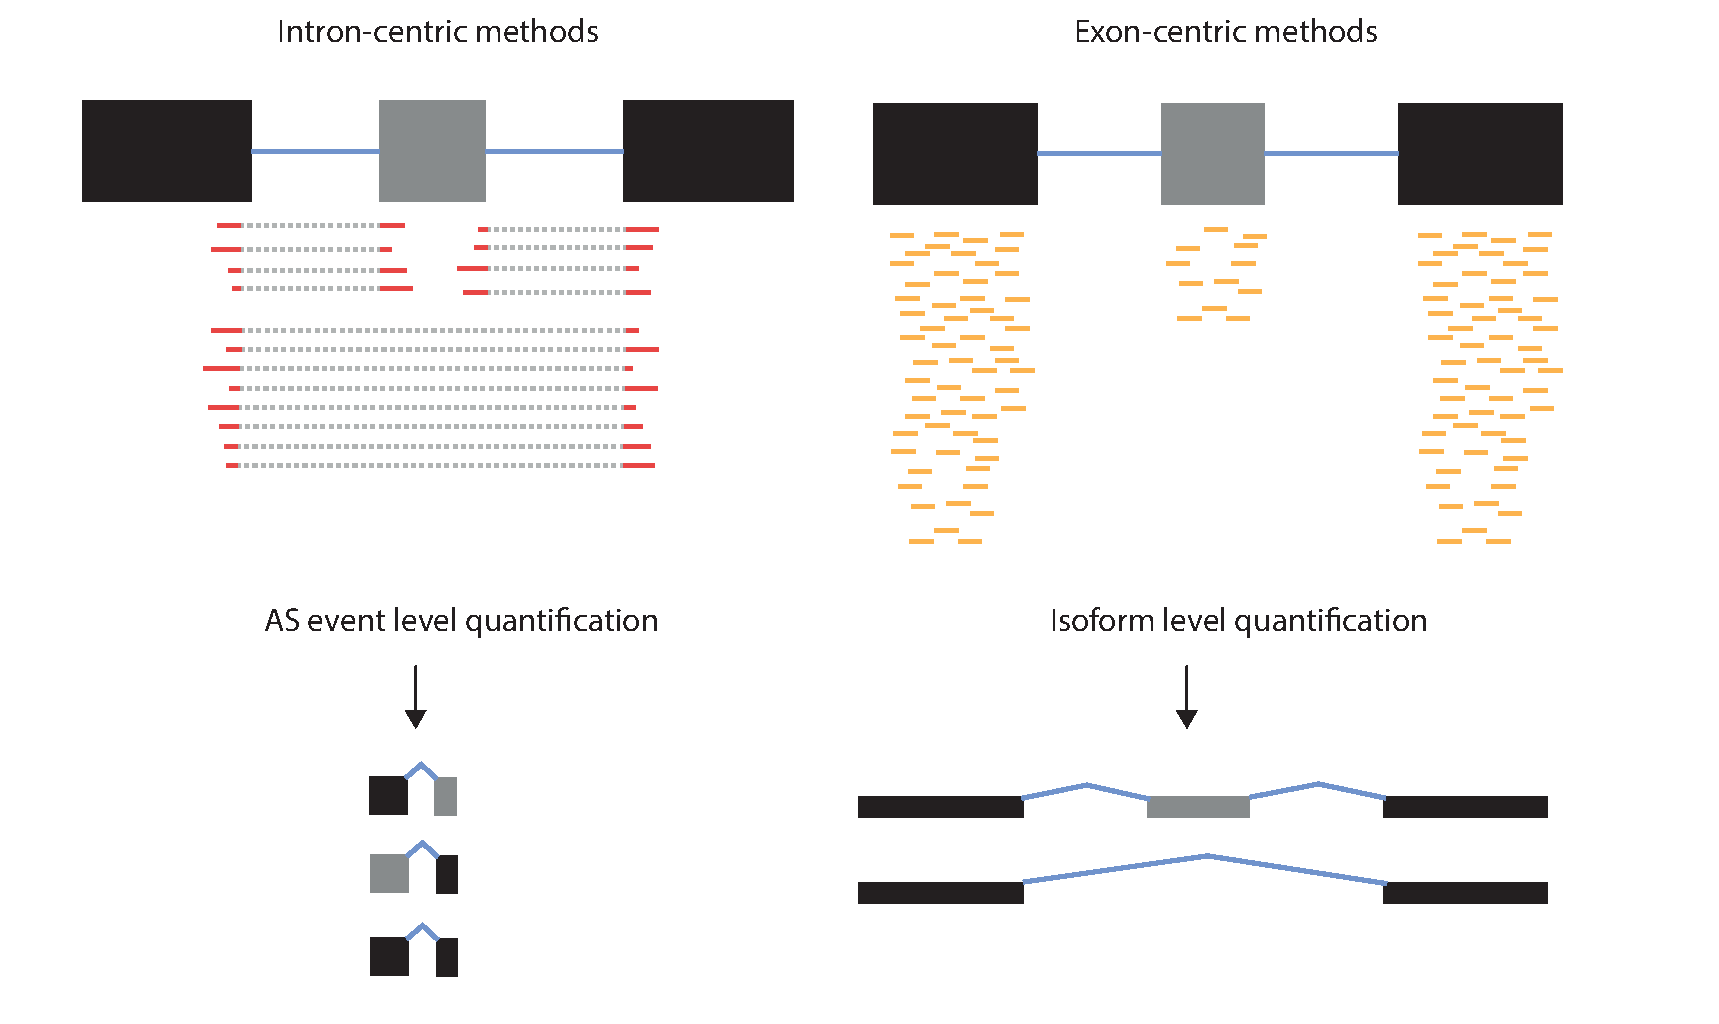
\includegraphics[width=\textwidth]{intron_exon_centric}
    \caption{}
    \label{fig:intron_exon_centric}   
  \end{figure}
AS quantification methods can be broadly divided into exon-centric and intron-centric methods. Exon-centric methods use exonic reads or a combination of exonic reads and reads spanning a splice junction (split reads) to infer isoform-level quantifications. These methods are heavily dependent on a known reference transcriptome, with some improvements to increase their ability to identify novel splice junctions \cite{Vaquero-Garcia2016-dv}. Their underlying assumption is that the relative abundance of exonic reads reflects the proportions of the unobserved isoforms. Conversely, intron-centric methods are based on the principle that AS proceeds in a step-wise fashion, where introns are excised from pre-mRNA. Instead of quantifyin AS via exonic reads, intron-centric methods use observed split reads at each splice junction to directly quantify local AS events. The obivious advantage of intron-centric method is that they provide less uncertain estimates of AS events as they do not attempt to provide probabilistic isoform-level quantifications. Moreover, they are able to detect novel splice junctions as they do not rely on a reference transcriptome to reconstruct isoforms. However, this comes at the cost of precision and interpretability. By definition, reads that span exon-intron-exon junctions are less abundant than exonic reads, as RNA-seq experiments typically sample mature mRNA transcripts. Consequently, intron-centric quantification methods such as Leafcutter build their AS quantification using much less reads than exon-centric methods such as MAJIQ, rMATS, or Cufflinks. Moreover, the interpretation of local AS events is usually less straightforward. Local AS events reflect local intron excision steps at each splice junctions, but it is often unclear how different intron excision events are connected to each other. \\

Leafcutter is an example of intron-centric AS quantification methods that use split reads to quantify local intron excision decisions (reads spanning splice junctions). To improve interpretability, local intron excision events are grouped into intron clusters. In its first pass, Leafcutter starts by pooling all observed split reads in all samples to identify a set of high-confidence 5' and 3' splice sites. In a second pass, Leafcutter counts the number of split reads that map to each intron identified in the first pass. Leafcutter then organises individual intron excision events into an undrirected graph structure. Nodes represent local intron excision events which are connected by edges. The Leafcutter algorithm connects two nodes (i.e. introns) if they share a 5' or 3' splice site. The overall Leafcutter procedure results in functionally connected groupings of introns called intron clusters. Within each intron cluster, intron usage is quantified as the proportion of all split reads that map to each individual intron. This final quantification is performed separately for each RNA-seq sample and the result is a matrix of intron usage ratio for all study samples. 

\subsection{Genetic regulation of alternative splicing}
AS is tightly regulated by several cis- and trans-acting factors. This tight regulation ensures splicing fidelity by correctly guiding the splicing machinery towards the target acceptor and donor splice sites, and by a complex interplay of splicing factors that promote and/or inhibit splicing. Despite the apparent complexity of the splicing code \cite{Jaganathan2019-ah}, direct mutagenesis as well as computational approaches have elucidated several cis-acting sequence elements that guide the choice of splice sites and improve spliceosomal efficiency. These include exonic splicing enhancers (ESE), exonic splicing silencer (ESS), intronic splicing enhancers (ISE) and intronic splicing silencers (ISS). Splicing regulatory elements mostly work by recruiting various classes of trans-acting splicing factors to their target splicing sites. These factors either promote or hinder the recruitment of the spliceosomal complex. Most ESEs are bound by members of the serine/arginine rich proteins (SR proteins), which enhance the recruitment of several snRNPs necessary to initiate the splicing process (reviewed in \cite{Shepard2009-os}). The promotion of splicing is often countered by the recruitment of heterogenous nuclear ribonucleoproteins (hnRNPs) to ESS, which often block the recruitment of the splicing machinery \cite{Geuens2016-yz}. The disruption of this tight regulation underpins several diseases. Spinal muscular atrophy, a debilitating motor neuron disease, is caused by the skipping of exon7 in \textit{SMN1}. Exon 7 skipping is caused by a single nucleotide substition that alters the ESE sequence and results in a non-functional \textit{SMN1} protein isoform \cite{Monani1999-vf}.\\

\subsection{Mapping sQTLs}

Given the complex regulatory network that underpins AS regulation, understanding the impact of genetic variation on AS patterns paves the pathway to understand the impact of AS dysregulation on human health. Moreover, understanding how AS patterns are regulated in relevant contexts can help us better understand the impact of disease-associate genetic variant on the transcriptome. Similar to expression QTLs, where genetic variants associated with gene abundance, AS quantifications can be used as a molecular trait to uncover the genetic determinant of AS (splicing QTLs). However, there are a few conceptual and methodological differences between sQTL mapping and eQTL mapping. \\

Depending the AS quantification method, the interpretation of sQTLs can vary. sQTLs discovered using isoform abundance as a molecular trait are the easiest to interpret. In this case, a significant sQTL would be defined as a genetic variant that increases or decreases a particular transcript abundance. This interpretation is less straightforward when AS is quantified at the AS event level. When intron usage ratios are used as quantitative trait, a significant sQTL can be defined as a variant that changes the proportion of a particular intron within its intron cluster. Therefore, when sQTLs are mapped using intron usage ratios, it is often helpful to examine the effect of the discovered genetic variant on all neighbouring AS events to build a more complete picture of the splicing event under investigation. For example, in Figure \ref{fig:intron_exon_centric}, upon examination of all three AS events in the left-hand panel, it becomes clear that the identified AS events represents an exon inclusion/skipping decision. Additionally, it is important to note that different AS events are often highly correlated. This is because intron usage ratios within an intron cluster always add up to 1. Therefore, genetic variants that lead to an increased usage of one intron also causes decreased usage of one or more other introns. As a result, it is often the case that within each intron cluster, multiple significant sQTLs do not necessarily represent distinct regulatory effects, but rather highly correlated measurements. 


\subsection{Comparing QTL effects in multiple conditions}
A long-standing question in QTL studies is how gene expression is genetically regulated in different tissues, cell types and environmental contexts. Answering this question is important to understand which transcriptomic effects of genetic variation are shared or distinct in different biological contexts. Context-dependence of QTL effects has often motivated multi-tissue QTL studies, with the assumption that profiling QTL effects in different contexts can draw a more complete picture of gene expression regulation. For example, in a comparison of eQTL effects between CD4+ T-cells and monocytes, Raj et al. \cite{Raj2014-xw} found that at least 42 genes had opposing eQTL effects in the two cell types. In line with this, Peters et al. \cite{Peters2016-zk} found that 87 genes had discordant eQTL effects in five different immune cell types. Although these dramatically discordant examples of genetic regulation represented a minority of eQTL effects, they demonstrate the impact that biological context on genetic regulation.\\

More generally, assessing the sharing of QTL effects in different treatment groups is non-trivial. In most QTL studies, QTL discovery is carried out separately for different treatment groups. This means that incomplete power may cause truly shared QTL effects to appear non-significant in some groups simply by chance. Direct comparison of effect sizes between different groups is therefore likely to overestimate the number of distinct QTL effects. To address this issue, several methods that probabilistically model effect sizes were developed \cite{Flutre2013-sp,Li2018-kr,Sul2013-xm, Urbut2019-gf}. Earlier methods were inspired by fixed-effects meta-analysis methods, and started from the assumption that any given eQTL effect is shared across all conditions. Later, methods that adapted this assumption to the data-driven correlation structure were developed. For example, multivariate adaptive shrinkage (mash) empirically learns the patterns of effect sharing in the dataset under study, and allows for arbitrary patterns of sharing between multiple conditions. For example, QTLs derived from different brain regions are expected to have highly correlated effect sizes. Usually, this correlation strucuture is learned from a random unbiased set of QTL effects (i.e. non-significant QTLs).\\

A Bayesian approach is then applied to re-estimate effect sizes for a desired set of QTL effects (e.g. significant QTL effects). The posterior effect sizes are then tested for evidence of effect size heterogeneity between different groups. The obious advantage of mash is that the re-estimated effect sizes take into account the empirical correlation structure in the dataset. However, this also means that significant QTL effects' sharing may be overestimated when the null QTL effects are highly correlated among the treatment groups. As a result, this may hide truly context-dependent QTL effects simply because there was not enough statistical power to suggest heterogeneity of effect sizes. Additionally, when the significant QTL effects are tested for condition-specificity, only the lead QTL SNP is used. In many cases, sharing of the lead QTL SNP does not necessarily mean that the underlying causal variant is shared between different conditions. It has been previously showing that comparing the lead SNP between different association signals can lead to the false conclusion that the effects under comparison are shared \cite{Liu2019-fv}. A better approach should leverage the linkage disequillibrium structure to assess if two association signals under comparison are likely to be shared or distinct. Nonetheless, mash can still be useful if the degree of QTL sharing is interpreted as an upper bound, rather than an accurate estimate of QTL sharing.\\


\subsection{Approaches to link to disease-associated GWAS loci to QTL effects}
In addition to understand gene regulation, a major objective of QTL studies is to integrate QTL effects with GWAS data. The simplest approach is to test the replication of the lead GWAS SNP in the QTL dataset. It is often compelling to assume that a replicated SNP may indicate that both gene expression and disease risk are driven by the same variant. In fact, lead SNP comparison was commonly used to implicate effector genes at many disease-associated loci. However, this direct SNP comparison was found to result in many false positives \cite{Liu2019-fv}. Threfore, more robust methods to compare pairs of association signals were developed to fill this gap. Particularly, statistical colocalisation methods take into account the association signal of all variants in a region to make a conclusion about a pair of association signals. Although the true causal variant may not be genotyped or imputed in either of the association studies, its effect is tagged by other variants in linkage disequillibrium with the true causal variant. Colocalisation methods leverages the linkage disequillbrium in a given locus to make an inference about two association signals. The underlying assumption is that if the two association signals are consistent across the region, it is likely that the same variant is driving both signals. Therefore, colocalisation results are only valid when the LD pattern is similar between the two association signals under comparison. This assumption only holds if the two association studies being compared are derived from population with the same ancestry, which is an important consideration when comparing two association signals. Additionally, standard colocalisation approaches only test the hypothesis that a \textit{single} shared variant underpins the two association signals. Many QTL studies have shown that for many genes secondary and even tertiary association signals are discovered for several genes, and the same observation applies to GWAS signals. Violations of the single causal variant assumption at loci with multiple causal variants will result in decreased power to detect true colocalisations. Therefore, extensions to standard colocalisation idenitfy independent association signal in each of the two cohorts, before proceeding to perform colocalisation analysis for each of the identified signals. This approach has been shown to increase the number of colocalised signals detected \cite{Wallace2021-rv}.\\  



\subsubsection{Colocalisation}

\subsubsection{Other approaches}

% Statistical modelling of effect sizes tests the alternative hypothesis that a given effect size is significantly different in one or more treatment groups. Different methods test this hypothesis in different ways. Earlier methods were inspired by fixed-effects meta-analysis approaches and 
% The complex regulatory network of cis-acting elements and trans-acting factors suggests that regulatory errors can arise 

% Since the 1970s, alternative splicing (AS) has emerged as an important post-transcriptional modification. AS has been shown to remarkably increase the coding potential of an otherwise fixed repertoire of genes. Through diversification of the transcriptome, AS contributes to phenotypic complexity in higher organisms. Previous work has shown that AS is more prevalent in higher eukaryotes compared to lower eukaryotes, and in vertebrates compared to invertebrates (10.1038/nrg2776). Our appreciation of the role of AS has also changed over time. Today, we know that 95% of multi-exonic genes are alternatively spliced, compared to an estimate of only 5-35% shortly after the Human Genome Project (https://www.hindawi.com/journals/ijeb/2012/596274/; https://www.ncbi.nlm.nih.gov/pmc/articles/PMC2443848/). 


\subsection{why we need qtl studies}
\subsection{why molecular qtls are context dependent - same dna - different gene expression}
\subsection{why is it important to understand disease-associated variants in a relevant context}
\subsection{the variety of molecular QTLs: caQTLs, histone marker QTLs..etc}
\subsection{Most studies have focussed on overall levels of gene expression}